% created on 19/11/2020
% @author : ebazan

\chapter{Similarity Measures of Distributions}\label{ch:similarity_measures}
Associated publications: \vspace{-2mm}

%\begin{itemize}
%	\item \citep{Bazan.Dokladal.ea:BMVC:2019}. << Quantitative Analysis of Similarity Measures of
%Distributions >>. In: \textit{30th British Machine Vision Conference 2019, BMVC 2019}. BMVC press, Cardiff, UK.
%\end{itemize}

\section*{Résumé}
\noindent Il existe de nombreuses mesures de dissemblance qui, selon l'application, n'ont pas toujours un comportement optimal. Dans ce chapitre, nous présentons une analyse qualitative des mesures de similarité les plus utilisées dans la littérature et de la Earth Mover's Distance (EMD). L'EMD est une métrique basée sur la théorie du transport optimal avec des propriétés géométriques intéressantes pour la comparaison des distributions. Cependant, l'utilisation de cette mesure est limitée par rapport à d'autres mesures de similitude. La raison principale était, jusqu'à récemment, la complexité du calcul. Nous montrons la supériorité de l'EMD à travers trois expériences différentes. Premièrement, analyser la réponse des mesures dans le plus simple des cas; distributions synthétiques à une dimension. Deuxièmement, avec deux systèmes de récupération d'images; en utilisant des fonctionnalités de couleur et de texture. Enfin, utiliser une technique de réduction dimensionnelle pour une représentation visuelle des textures. Nous montrons qu'aujourd'hui l'EMD est une mesure qui reflète mieux la similitude entre deux distributions.

\section*{Abstract}
\noindent There are many measures of dissimilarity that, depending on the application, do not always have optimal behavior. In this chapter, we present a qualitative analysis of the similarity measures most used in the literature and the Earth Mover's Distance (EMD).  The EMD is a metric based on the theory of optimal transport with interesting geometrical properties for the comparison of distributions. However, the use of this measure is limited in comparison with other similarity measures. The main reason was, until recently, the computational complexity. We show the superiority of the EMD through three different experiments. First, analyzing the response of the measures in the simplest of cases; one-dimension synthetic distributions. Second, with two image retrieval systems; using color and texture features. Finally, using a dimensional reduction technique for a visual representation of the textures. We show that today the EMD is a measure that better reflects the similarity between two distributions.

\section{Introduction}\label{sec:introduction}
In image processing and computer vision, the comparison of distributions is a frequently used technique. Some applications where we use these measures are image retrieval, classification, and matching systems \citep{Smeulders.Worring.ea:PAMI:2000}. For these, the distributions could represent low-level features like pixel's intensity level, color, texture or higher-level features like objects. The comparison could be done using a unique feature, for example, the texture \citep{Banerjee.Bhunia.ea:ESWA:2018, Kwitt.Uhl:ICIP:2008}, or combining features in a multi-dimensional distribution as the fusion of color and texture features \citep{Liu.Guo.ea:IS:2017}. In the field of medical imaging, comparing distributions are useful to achieve image registration \citep{So.Chung:JPR:2017}. More general applications such as object tracking \citep{Nejhum.Ho.ea:CVPR:2008, Klein.Frintrop:CV:2011} and  saliency modeling \citep{Bylinskii.Judd.ea:PAMI:2018}, also use the comparison of distributions. Regarding the number of computer vision applications that make use of the comparison of distributions, the choice of the correct metric to measure the similarity between distributions is crucial. 

The Earth Mover's Distance (EMD) \citep{Rubner.Tomasi.ea:IJCV:2000} is a dissimilarity measure inspired by the optimal transport theory. This measure is considered as true distance because it complies with the constraints of non-negativity, symmetry, identity of indiscernibles, and triangle inequality \citep{Peyre.Cuturi:arXiv:2018}. The superiority of the EMD over other measures has been demonstrated in several comparative analysis (see for example \citep{Puzicha.Buhmann.ea:ICCV:1999, Rubner.Tomasi.ea:IJCV:2000}). Despite this superiority in theory, in practice, this distance continues to be underused for the benefit of other measures. The main reason is the high computational cost due to its iterative optimization process. However, nowadays this should not be a problem thanks to the algorithmic advances to computing efficiently the EMD (see ``Notes about EMD computation complexity'' in section \ref{sec:conclusions}) and the progress of computer processors. Although there are comparative studies (image retrieval scores, for example), in this paper, we illustrate how other similarity measures dramatically fail even on very simple tasks. We use a set of 1D synthetic distributions and two simple image databases (color and texture-based) to compare a set of similarity measures through two image retrieval systems and a visual representation in low-dimensional spaces. We show that, surprisingly, no metric but the EMD yields to classify and give a coherent visual representation of the images of the databases (see Figs. \ref{fig:superman_distances} and \ref{fig:wonderwoman_distances} in the supplementary material file). In this paper, we want to emphasize the importance of having a true metric to measure the similarity between distributions.

In this chapter, we present a new qualitative study of some popular similarity measures. Our primary objective is to show that not all measures express the difference between distributions adequately. Also, we show that today the EMD is a competitive measure concerning computing time. Among the similarity measures that we compare are some of the most used bin-to-bin class methods; the histogram intersection and correlation \citep{Nejhum.Ho.ea:CVPR:2008}, the Bhattacharya distance \citep{So.Chung:JPR:2017}, the $\chi^2$ statistic and, the  Kullback-Leibler divergence \citep{Klein.Frintrop:CV:2011}. 

This chapter is organized as follows: in section \ref{sec:measures}, we describe and discuss some properties of the bin-to-bin measures and we expose the geometrical properties of the EMD. Then, in section \ref{sec:comparison}, we show the performance of the different similarity measures with a one-dimensional test, with two image classifiers; one based on color (3D case) and other based on texture (2D case) information and, with a dimensionality reduction using the multidimensional scaling (MDS) technique. Finally, in section \ref{sec:conclusions}, we close this chapter with some reflections about EMD and optimal transport in the field of image processing and computer vision.


\section{Similarity Measures Review}\label{sec:measures}

\paragraph{Similarity Measures Notation.}
In many different science fields, there is a substantial number of ways to define the proximity between distributions. In abuse of language, the use of synonyms such as \textit{similarity}, \textit{dissimilarity}, \textit{divergence} and, \textit{distance}, complicates the interpretation of such a measure. Here we recall a coherent notation, used throughout this chapter.

A \textbf{\textit{distance}}, from the physical point of view, is defined as a quantitative measurement of how far apart two entities are. Mathematically, a distance is a function $d : M \times M \rightarrow \mathbb{R}^+$. We say that $d$ is a \textbf{\textit{true distance}} if $\forall (x, y) \in M \times M$ it fulfills the following properties.

\begin{enumerate}%[noitemsep]%,topsep=0pt
 \item Non-negativity: $d(x, y)\geq 0$
 \item Identity of indiscernibles: $d(x, y) = 0$ if and only if $x = y$
 \item Symmetry: $d(x, y) = d(y, x)$
 \item Triangle inequality: $d(x, y) \leq d(x, z) + d(z, y)$
\end{enumerate}

From this definition, we can define other distances depending on which properties are (or not) fulfilled. For example, \textbf{\textit{pseudo-distances}} do not fulfill the identity of indiscernibles criterion; \textbf{\textit{quasi-distances}} do not satisfy the symmetry property; \textbf{\textit{semi-distances}} do not fulfill the triangle inequality condition; and \textbf{\textit{divergences}} do not comply with the last two criteria~\citep{Khamsi:JFPTA:2015}.

According to the measure, the numerical result could represent the similarity or the dissimilarity between two distributions. The \textbf{\textit{similarity}} and the \textbf{\textit{dissimilarity}} represent, respectively, how alike or how different two distributions are. Namely, a similarity value is higher when the distributions are more alike while a dissimilarity value is lower when the distributions are more alike. In this paper we use the term \textbf{\textit{similarity}} to refer either how similar or how dissimilar two distributions are. If distributions are close, they will have high similarity and if distributions are far, they have low similarity. 
 
\subsection{Bin-to-Bin Similarity Measures}
In computer vision, distributions describe and summarize different features of an image. These distributions are discretized by dividing their underlying support into consecutive and non-overlapping bins $p_i$ to generate histograms. Let $\mathbf{p}$ be a histogram which represents some data distribution. In the histogram, each bin represents the mass of the distribution that falls into a certain range; the values of the bins are non-negative reals numbers. 

The bin-to-bin measures compare only the corresponding bins of two histograms. Namely, to compare the histograms  $\mathbf{p} = \{p_i\}$ and $\mathbf{q} = \{q_i\}$, these techniques only measure the difference between the bins that are in the same interval of the feature space, that is, they only compare bins  $p_i$ and $q_i$ $\forall i=\{1, \ldots, n\}$, where $i$ is the histogram bin number and $n$ is total number of bins. The Table \ref{table:b2b_eqs} summarizes the bin-to-bin measures we compare.

The \textbf{histogram intersection} \citep{Swain.Ballard:IJCV:1991} is expressed by a \textit{min} function that returns the smallest mass of two input bins (see Eq. \ref{eq:hist_inter}). As a result, the measure gives the number of samples of $\mathbf{q}$ that have corresponding samples in the $\mathbf{p}$ distribution. According to the notation defined at the beginning of section \ref{sec:measures}, the histogram intersection is a similarity measure.
\begin{eqnarray}
d_{\cap}(\mathbf{p}, \mathbf{q}) = 1 - \frac{\sum_{i}\min(p_i, q_i)}{\sum_{i}q_i} \label{eq:hist_inter}
\end{eqnarray}

The \textbf{histogram correlation} gives a single coefficient which indicates the degree of relationship between two variables. Derived from the Pearson's correlation coefficient, this measure is the covariance of the two variables divided by the product of their standard deviations. In Eq. \ref{eq:hist_corr}, $\overline{\mathbf{p}}$ and $\overline{\mathbf{q}}$ are the histogram means. Since this measure is a pseudo-distance (the resulting coefficient is between -1 and 1), it expresses the similarity of the distributions.  
\begin{eqnarray}
d_{C}(\mathbf{p}, \mathbf{q}) = \frac{\sum_{i}(p_i - \overline{\mathbf{p}})(q_i - \overline{\mathbf{q}})}{\sqrt{\sum_{i}(p_i - \overline{\mathbf{p}})^{2}\sum_{i}(q_i - \overline{\mathbf{q}})^{2}}} \label{eq:hist_corr}
\end{eqnarray}

The \textbf{$\chi^2$ statistic} measure comes from the Pearson's statistical test for comparing discrete probability distributions. The calculation of this measure is quite straightforward and intuitive. As depicted in Eq. \ref{eq:chi_square}, the measure is based on the difference between what is actually observed and what would be expected if there was truly no relationship between the distributions. From a practical point of view, it gives the dissimilarity between two distributions.
\begin{eqnarray}
d_{\chi^2}(\mathbf{p},\mathbf{q}) = \sum\nolimits_i \frac{(p_i - q_i)^2}{q_i} \label{eq:chi_square}
\end{eqnarray}

% NOTE: See the second opencv implemetationin of the chi squared distance that use m_i, where $m_i = \frac{p_i + q_i}{2}$

The \textbf{Bhattacharyya distance} \citep{Bhattacharyya:IJS:1946} is a pseudo-distance which is closely related to the Bhattacharyya coefficient. This coefficient, represented by $\sum_i\sqrt{p_{i}q_{i}}$ in Eq. \ref{eq:bhatt_dist}, gives a geometric interpretation as the cosine of the angle between the distributions. We normalize the values of this measure between 0 and 1 to express the dissimilarity between two distributions.
\begin{eqnarray}
d_{B}(\mathbf{p}, \mathbf{q}) = \sqrt{1- \frac{1}{\sqrt{\overline{\mathbf{p}} \overline{\mathbf{q}} n^2}} \sum\nolimits_{i} \sqrt{p_i q_i}} \label{eq:bhatt_dist}
\end{eqnarray}

The \textbf{Kullback-Leibler divergence} \citep{Kullback.Leibler:IMS:1951}  measures the difference between two histograms from the information theory point of view. It gives the relative entropy of $\mathbf{p}$ with respect to $\mathbf{q}$ (see Eq. \ref{eq:kl_div}). Although this measure is one of the most used to compare two distributions, it is not a true metric since it does not fulfill the symmetry and the triangle inequality properties described in section \ref{sec:measures}.
\begin{eqnarray}
d_{KL}(\mathbf{p}, \mathbf{q}) = \sum\nolimits_{i}p_i \log\frac{p_i}{q_i} \label{eq:kl_div}
\end{eqnarray}

We can find other measures in the literature that represent the similarity between distributions, for example, the \textbf{Lévy–Prokhorov metric} \citep{Prokhorov:TPA:1956} and the \textbf{total variation distance} \citep{Bogachev.Kolesnikov:RMS:2012}. The first one defines the distance between two probability measures on a metric space with its Borel sigma-algebra. However, the use of this is not very frequent in the area of computer vision because of the implementation complexity \citep{Bogachev.Kolesnikov:RMS:2012}. The second one equals the optimal transport distance \citep{Cuturi.Avis:JMLR:2011} in the simplified setup when the cost function is $c(x,y)=1, x\neq y$. For countable sets, it is equal to the $L_1$ norm. Taking this into account, we only use the first five bin-to-bin measures defined in the following experiments.
\begin{eqnarray}
d_{TV}(\mathbf{p}, \mathbf{q}) = \frac{1}{2}\sum\nolimits_{i}|p_i - q_i | \label{eq:tv_dist}
\end{eqnarray}


\subsection{The Earth Mover's Distance}\label{subsec:EMD}
Earth Mover's Distance is the term used in the image processing community for the optimal transport; in other areas, we also find this measure referred to as the Wasserstein distance \citep{Gibbs.Su:ISR:2002} or the Monge-Kantorovich problem \citep{Bogachev.Kolesnikov:RMS:2012, Kantorovich:JMS:2006}. This concept lays in the study of the transportation theory which aims for the optimal transportation and allocation of resources. 
The main idea behind the optimal transport is simple and very natural for the comparison of distributions. Let
$
\boldsymbol{\alpha} = \sum_{i=1}^{n}\alpha_{i}\delta_{x_i} \text{  and  } \boldsymbol{\beta} = \sum_{j=1}^{m}\beta_{j}\delta_{y_j}
$
be two discrete measures supported in $\{x_1, \ldots, x_n\} \in \mathcal{X}$ and $\{y_1, \ldots, y_n\} \in \mathcal{Y}$, where $\alpha_i$ and $\beta_j$ are the weights of the histograms bins $\boldsymbol{\alpha}$ and $\boldsymbol{\beta}$; $\delta_{x_i}$ and $\delta_{y_j}$ are the Dirac functions at position $x$ and $y$, respectively. Intuitively, the Dirac function represents a unit of mass which is concentrated at location $x$. This notation is equivalent to the one proposed in \citep{Rubner.Tomasi.ea:IJCV:2000} where $\delta_{x_i}$ is the central value in bin $i$ while $\alpha_i$ represents the number of samples of the distribution that fall in the interval indexed by $i$.

%$\mathbf{C}_{ij} = c(x_i, y_i)$
The key elements to compute the optimal transport are the cost matrix $\mathbf{C} \in \mathbb{R}^{n\times m}_+$ , which define all pairwise costs between points in the discrete measures $\alpha$ and $\beta$, and the flow matrix (optimal transport matrix) $\mathbf{F} \in \mathbb{R}^{n\times m}_+$, where $f_{ij}$ describes the amount of mass flowing from bin $i$ (or point $x_i$) towards bin $j$ (or point $x_j$). Then the optimal transport problem consists in finding a total flow $\mathbf{F}$ that minimizes the overall cost defined as
\begin{eqnarray}
W_{\mathbf{C}}(\boldsymbol{\alpha}, \boldsymbol{\beta}) = \min \langle\mathbf{C},\mathbf{F}\rangle = \sum\nolimits_{ij} c_{ij}f_{ij}
\label{eq:optimal_work}
\end{eqnarray}

Placing the optimal transport problem in terms of \textit{suppliers} and \textit{consumers}; for a supplier $i$, at some location $\delta_{x_i}$, the objective is to supply $\alpha_i$ quantity of goods. On the other hand, a consumer $j$, at some location $\delta_{y_j}$, expects to recieve at most $\beta_j$ quantity of goods. Then, the optimal transport problem is subject to three constraints, $\forall i \in\{1, \ldots, n\}$, $j \in\{1, \ldots, m\}$

\begin{enumerate}%[noitemsep,topsep=0pt]%
 \item Mass transportation (positivity constraint): $f_{ij} \geq 0 : i\rightarrow j$.
 \item Mass conservation (equality constraint):  $\sum_{j}f_{ij}=\alpha_i$ and $\sum_{i}f_{ij}= \beta_j$.
 \item Optimization constraint: $\sum_{ij}f_{ij} = \min \left( \sum_{i}\alpha_i, \sum_{j}\beta_j \right)$ .
\end{enumerate}  

Then, we define the Earth Mover's Distance as the work $W_{\mathbf{C}}$ normalized by the total flow
\begin{eqnarray}
d_{EMD}(\boldsymbol{\alpha}, \boldsymbol{\beta}) = \frac{\sum_{ij}c_{ij}f_{ij}}{\sum_{ij}f_{ij}}
\label{eq:emd}
\end{eqnarray}

The importance of the EMD is that it represents the distance between two discrete measures (distributions) in a natural way. Moreover, when we use a \textit{ground distance} as the cost matrix $\mathbf{C}$, the EMD is a true distance. Peyré and Cuturi \citep{Peyre.Cuturi:arXiv:2018} show the metric properties of the EMD. To show these advantages, we developed a series of experiments described in the next section.



\section{Comparative Analysis of Similarity Measures}\label{sec:comparison}

\subsection{One-Dimensional Case Study}\label{subsec:1d_case}
To compare the measures described in section \ref{sec:measures} in the simplest scenario, we use a set of one-dimensional synthetic distributions. We create a source distribution and a series of target distributions (see Fig. \ref{fig:source_target_dist}). Both, source and target distributions, has 1000 samples and are random normal distributions. The unique difference between them is that the mean of the target distributions ($\mu$) is increasing five units with respect to the previous distribution.

\begin{figure}[ht] 
	\centering
	\begin{subfigure}[b]{0.45\textwidth}
		\centering
		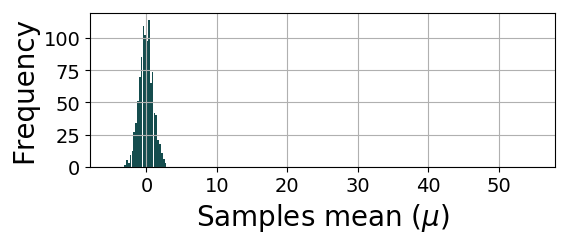
\includegraphics[width=\textwidth]{source_distribution}	
		\label{fig:source_distribution}
	\end{subfigure}
	~ %add desired spacing between images, e. g. ~, \quad, \qquad, \hfill etc. 
	%(or a blank line to force the subfigure onto a new line)
	\begin{subfigure}[b]{0.45\textwidth}
		\centering
		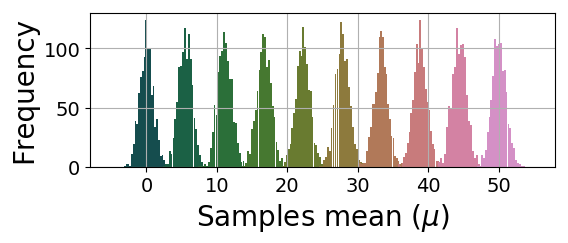
\includegraphics[width=\textwidth]{target_distributions}	
		\label{fig:targert_distributions}
	\end{subfigure}

  \caption{Source and target synthetic distributions}
  \label{fig:source_target_dist}
\end{figure}


\begin{figure}[!ht]
    \centering
    \begin{subfigure}[b]{0.3\textwidth}
		\centering
		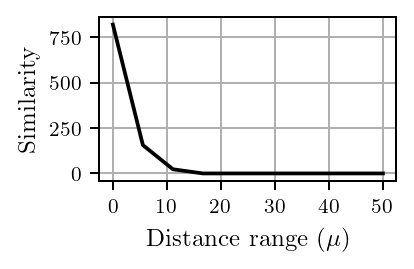
\includegraphics[width=\textwidth]{Inter_dist}	
		\caption{Histogram intersection}
        \label{fig:inter_dist}
	\end{subfigure}
	~ %add desired spacing between images, e. g. ~, \quad, \qquad, \hfill etc. 
    %(or a blank line to force the subfigure onto a new line)
    \begin{subfigure}[b]{0.3\textwidth}
		\centering
		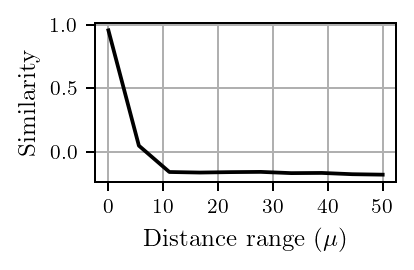
\includegraphics[width=\textwidth]{Corr_dist}	
		\caption{Histogram correlation}
        \label{fig:corr_dist}
	\end{subfigure}
    ~ %add desired spacing between images, e. g. ~, \quad, \qquad, \hfill etc. 
    %(or a blnk line to force the subfigure onto a new line)
    \begin{subfigure}[b]{0.3\textwidth}
		\centering
		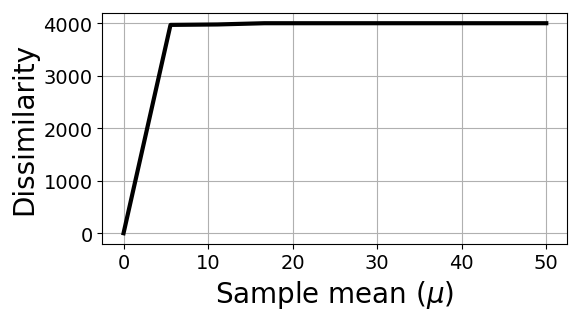
\includegraphics[width=\textwidth]{Chi2_dist}	
		\caption{$\chi^2$ Statistic}
        \label{fig:chi_square}
	\end{subfigure}  \\[2ex]
	
	
	\begin{subfigure}[b]{0.3\textwidth}
		\centering
		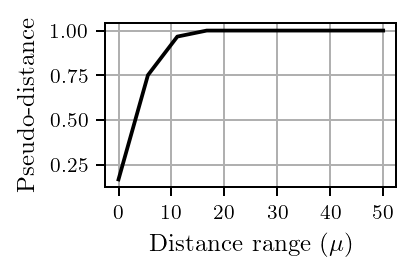
\includegraphics[width=\textwidth]{Bhatt_dist}	
		\caption{Bhattacharyya}
        \label{fig:bhatt_dist}
	\end{subfigure}
	~ %add desired spacing between images, e. g. ~, \quad, \qquad, \hfill etc. 
    %(or a blank line to force the subfigure onto a new line)    
    \begin{subfigure}[b]{0.3\textwidth}
		\centering
		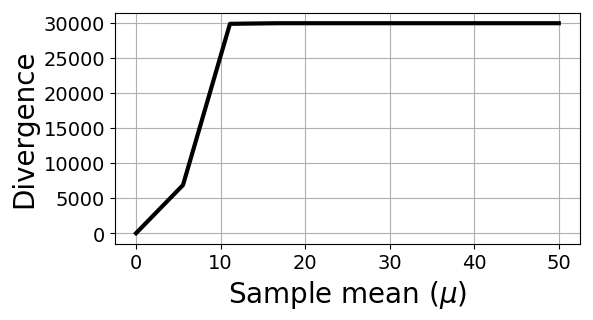
\includegraphics[width=\textwidth]{KL_dist}	
		\caption{Kullback-Leibler}
        \label{fig:kl_div}
	\end{subfigure}
    ~ %add desired spacing between images, e. g. ~, \quad, \qquad, \hfill etc. 
    %(or a blank line to force the subfigure onto a new line)
    \begin{subfigure}[b]{0.3\textwidth}
		\centering
		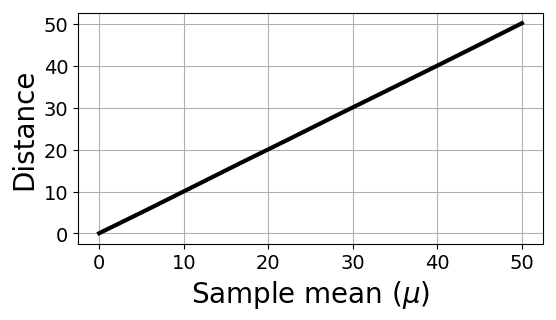
\includegraphics[width=\textwidth]{EMD_dist}	
		\caption{EMD}
        \label{fig:emd}
	\end{subfigure}
   
   \caption{Distances between the source and target distributions}
   \label{fig:distances}
\end{figure}

Since the distributions' mean value increases linearly, we expect that the similarity measure has an equivalent response, i.e., that the similarity decreases when the difference of the source and target means increases. In Fig. \ref{fig:distances}, we can see the response of the bin-to-bin measures and the EMD. Among the bin-to-bin measures, those that give a coefficient of dissimilarity ($\chi^2$ statistic, Bhattacharyya pseudo-distance and K-L divergence) rapidly saturate and stick to a maximum value; while for those that give a coefficient of similarity (histogram correlation and intersection), their value falls rapidly to zero. We can interpret these behaviors as follows. When the bins $p_i$, $q_i$ do not have any mass in common, the bin-to-bin measures fail in taking into account the mutual distance of the bins. They could consider that the distributions are precisely at the same distance (there is no difference between them), or that the distributions are entirely dissimilar. The only measure that presents a convenient behavior with the increasing difference of the means is the EMD. This is due to taking into account the \textit{ground distance} $\mathbf{C}$ of the matching bins (see above, Eq. \ref{eq:emd}). One can argue that for applications like image retrieval finding the most similar distribution is sufficient to find the alike image, or texture, whereas the ordering on the other ones is irrelevant. In the following experiment, we show that this intuition is incorrect and that even in an overly simple case the bin-to-bin measures are not the best choice.
 
\subsection{Image Retrieval Systems}
We develop two image retrieval systems as a second comparison test, one based on color information and the other based on texture information. For the classifiers, we use different databases. The first one contains 24 different color images of superhero toys\footnote{CC superheros images courtesy of Christopher Chong on Flickr}. It has 12 classes with two samples per class. The two first rows in Fig. \ref{fig:databases} show some examples of the superhero toys and their variations (change of the angle of the toy or the addition of accessories). The second database \citep{Kylberg:Dataset:2011} is composed of images belonging to different surfaces and materials (see the last two rows in Fig. \ref{fig:databases}). The database contains 28 different classes; it contains different patches per class. 

\begin{figure}[!ht]
	\centering
	\begin{subfigure}[b]{0.12\textwidth}
		\centering
		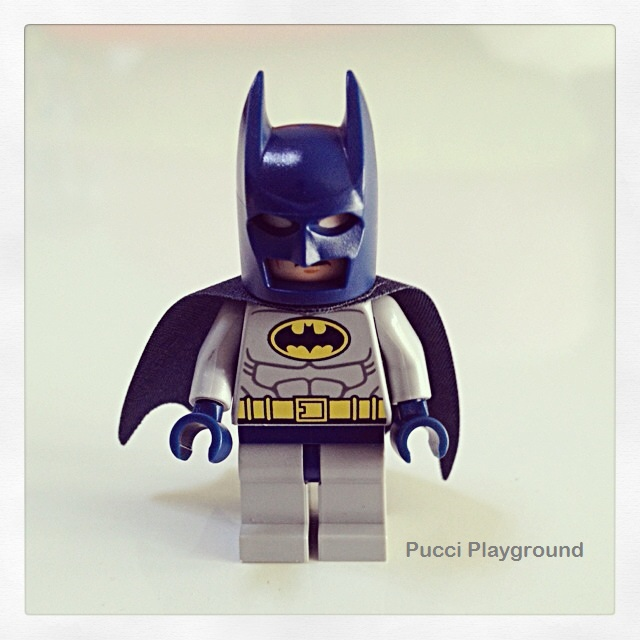
\includegraphics[width=\textwidth]{batman1_model}	
	\end{subfigure}
	~ %add desired spacing between images, e. g. ~, \quad, \qquad, \hfill etc. 
    %(or a blank line to force the subfigure onto a new line)
    \begin{subfigure}[b]{0.12\textwidth}
		\centering
		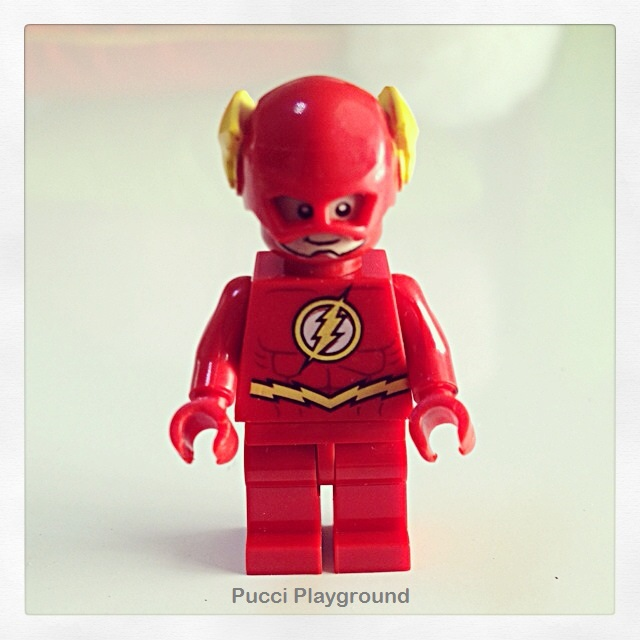
\includegraphics[width=\textwidth]{flash_model}	
	\end{subfigure}
    ~ %add desired spacing between images, e. g. ~, \quad, \qquad, \hfill etc. 
    %(or a blank line to force the subfigure onto a new line)
    \begin{subfigure}[b]{0.12\textwidth}
		\centering
		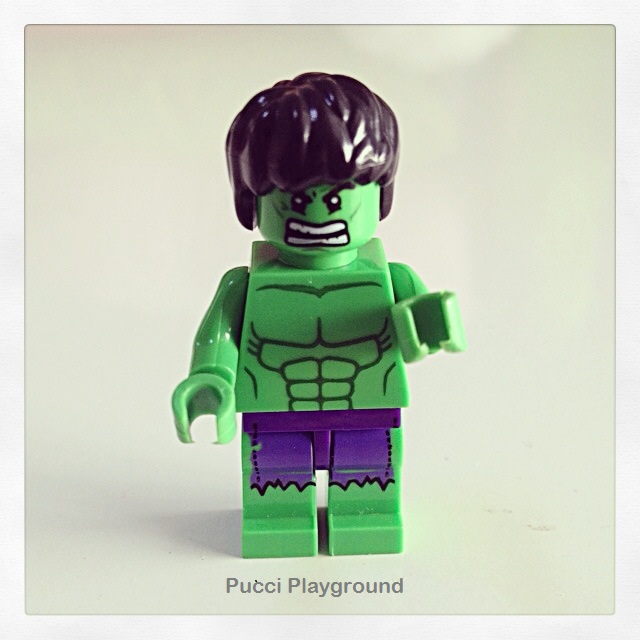
\includegraphics[width=\textwidth]{hulk_model}	
	\end{subfigure}
	~ %add desired spacing between images, e. g. ~, \quad, \qquad, \hfill etc. 
    %(or a blank line to force the subfigure onto a new line)
    \begin{subfigure}[b]{0.12\textwidth}
		\centering
		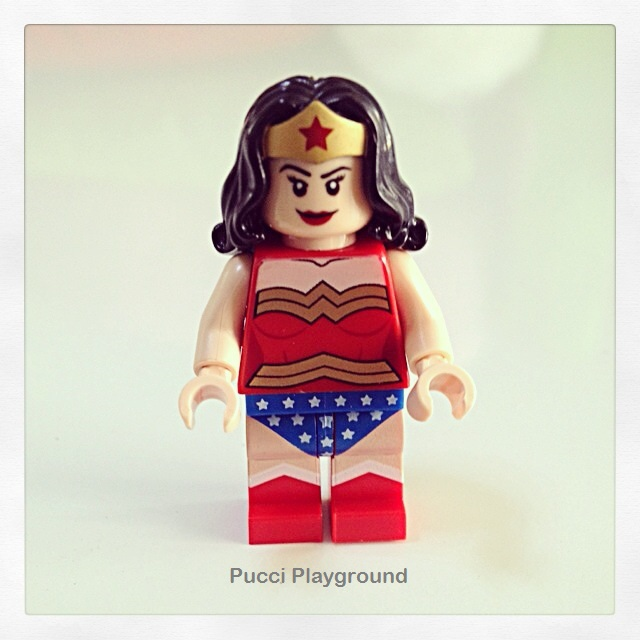
\includegraphics[width=\textwidth]{wonderwoman_model}	
	\end{subfigure}
    ~ %add desired spacing between images, e. g. ~, \quad, \qquad, \hfill etc. 
    %(or a blank line to force the subfigure onto a new line)
    \begin{subfigure}[b]{0.12\textwidth}
		\centering
		
\includegraphics[width=\textwidth]{wolverine_model}	
	\end{subfigure}
    ~ %add desired spacing between images, e. g. ~, \quad, \qquad, \hfill etc. 
    %(or a blank line to force the subfigure onto a new line)
    \begin{subfigure}[b]{0.12\textwidth}
		\centering
		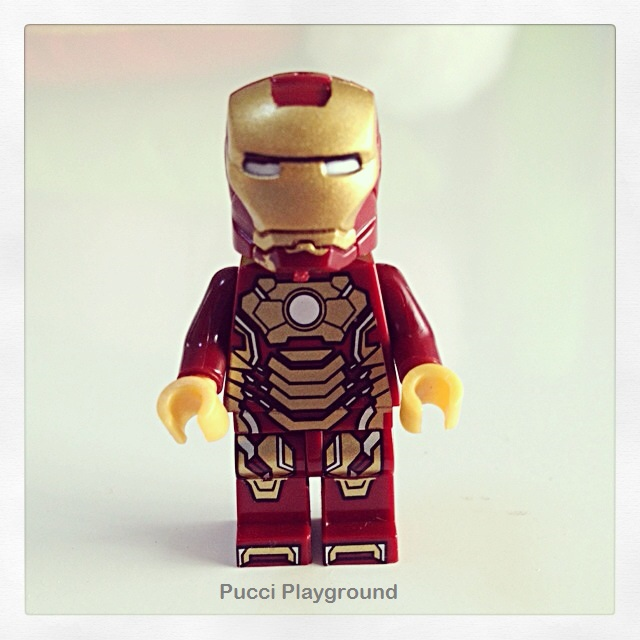
\includegraphics[width=\textwidth]{ironman_model}	
	\end{subfigure}
    ~ %add desired spacing between images, e. g. ~, \quad, \qquad, \hfill etc. 
    %(or a blank line to force the subfigure onto a new line)
    \begin{subfigure}[b]{0.12\textwidth}
		\centering
		
\includegraphics[width=\textwidth]{thor_model}	
	\end{subfigure} \\[2ex]
    
        
    \begin{subfigure}[b]{0.12\textwidth}
		\centering
		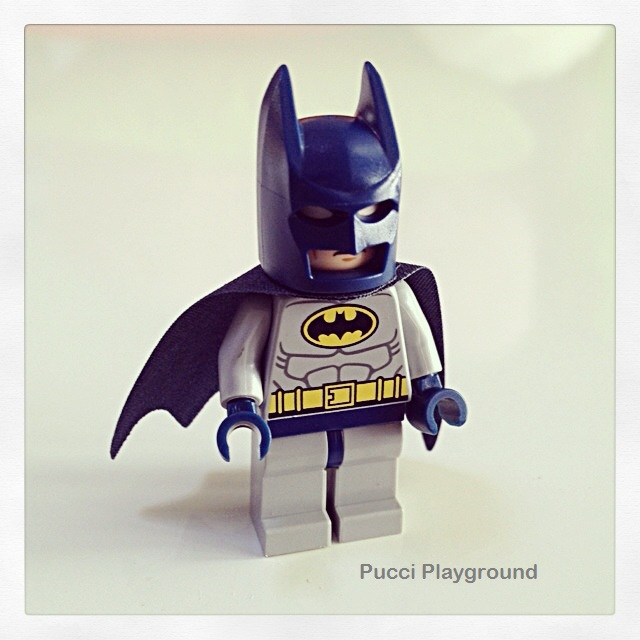
\includegraphics[width=\textwidth]{batman1}	
	\end{subfigure}
	~ %add desired spacing between images, e. g. ~, \quad, \qquad, \hfill etc. 
    %(or a blank line to force the subfigure onto a new line)
    \begin{subfigure}[b]{0.12\textwidth}
		\centering
		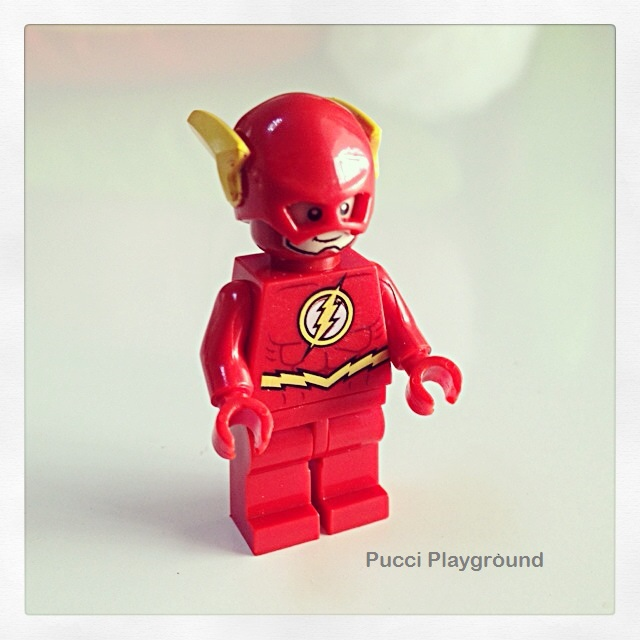
\includegraphics[width=\textwidth]{flash}	
	\end{subfigure}
    ~ %add desired spacing between images, e. g. ~, \quad, \qquad, \hfill etc. 
    %(or a blank line to force the subfigure onto a new line)
    \begin{subfigure}[b]{0.12\textwidth}
		\centering
		
\includegraphics[width=\textwidth]{hulk}	
	\end{subfigure}
	~ %add desired spacing between images, e. g. ~, \quad, \qquad, \hfill etc. 
    %(or a blank line to force the subfigure onto a new line)
    \begin{subfigure}[b]{0.12\textwidth}
		\centering
		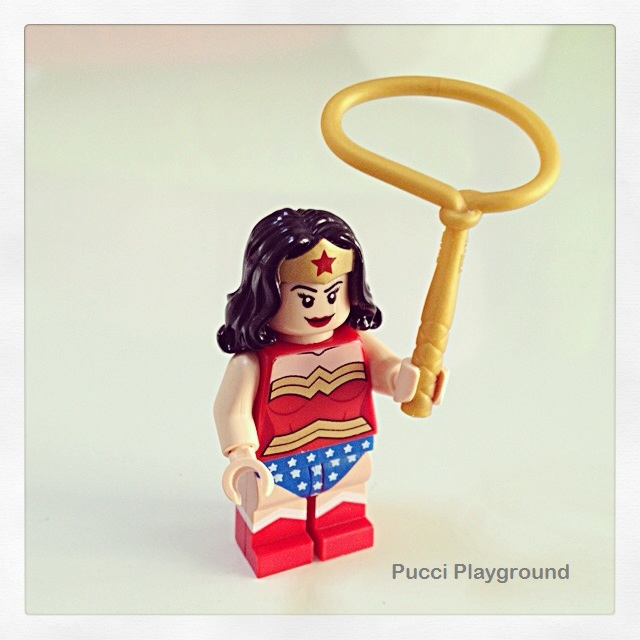
\includegraphics[width=\textwidth]{wonderwoman}	
	\end{subfigure}
    ~ %add desired spacing between images, e. g. ~, \quad, \qquad, \hfill etc. 
    %(or a blank line to force the subfigure onto a new line)
    \begin{subfigure}[b]{0.12\textwidth}
		\centering
		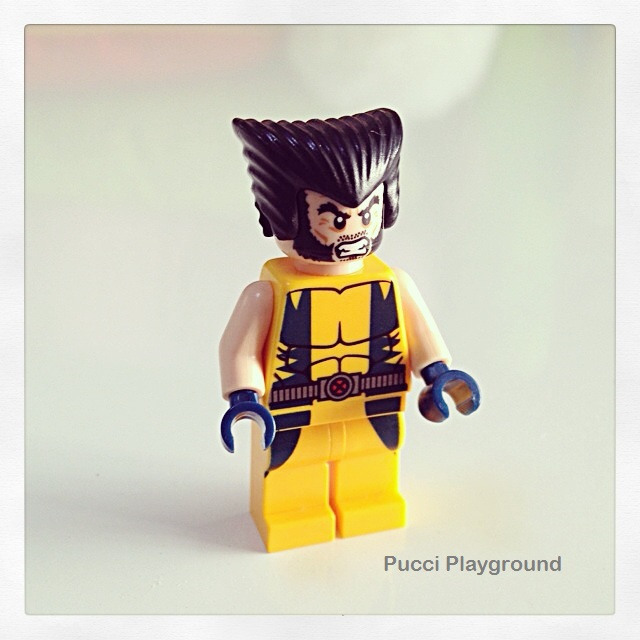
\includegraphics[width=\textwidth]{wolverine}	
	\end{subfigure}
    ~ %add desired spacing between images, e. g. ~, \quad, \qquad, \hfill etc. 
    %(or a blank line to force the subfigure onto a new line)
    \begin{subfigure}[b]{0.12\textwidth}
		\centering
		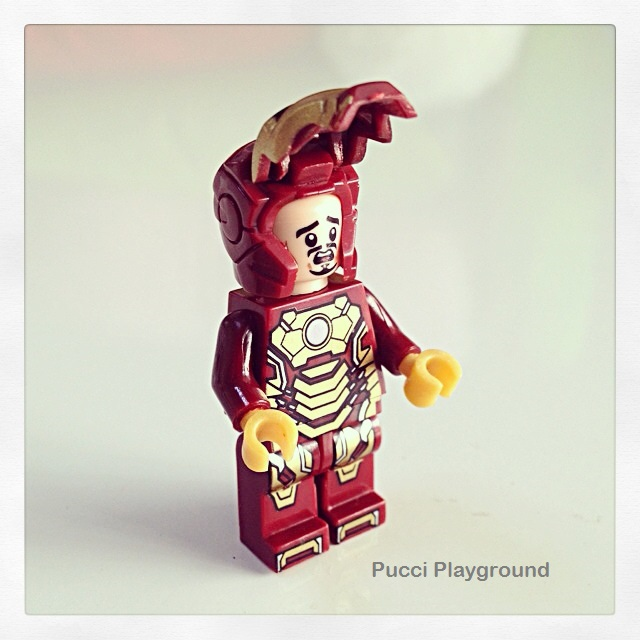
\includegraphics[width=\textwidth]{ironman_b}	
	\end{subfigure}
    ~ %add desired spacing between images, e. g. ~, \quad, \qquad, \hfill etc. 
    %(or a blank line to force the subfigure onto a new line)
    \begin{subfigure}[b]{0.12\textwidth}
		\centering
		
\includegraphics[width=\textwidth]{thor}	
	\end{subfigure} \\[2ex]
    
    
    \begin{subfigure}[b]{0.12\textwidth}
		\centering
		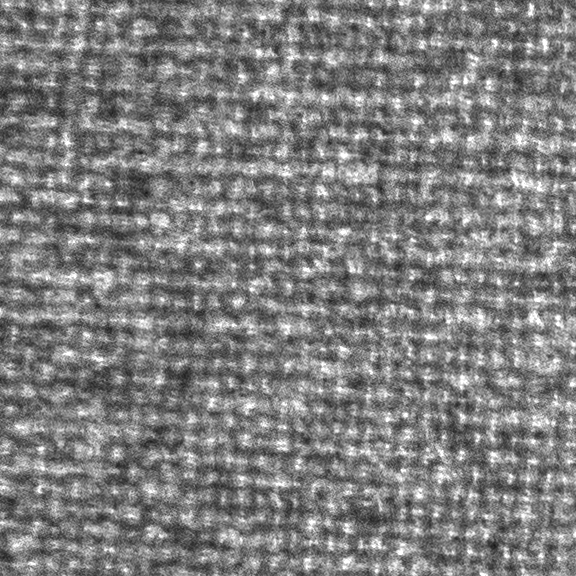
\includegraphics[width=\textwidth]{blanket1}	
	\end{subfigure}
	~ %add desired spacing between images, e. g. ~, \quad, \qquad, \hfill etc. 
    %(or a blank line to force the subfigure onto a new line)
    \begin{subfigure}[b]{0.12\textwidth}
		\centering
		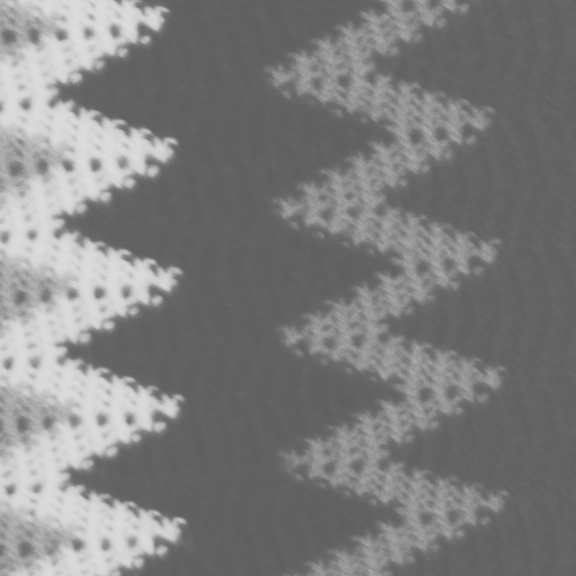
\includegraphics[width=\textwidth]{blanket2}	
	\end{subfigure}
    ~ %add desired spacing between images, e. g. ~, \quad, \qquad, \hfill etc. 
    %(or a blank line to force the subfigure onto a new line)
    \begin{subfigure}[b]{0.12\textwidth}
		\centering
		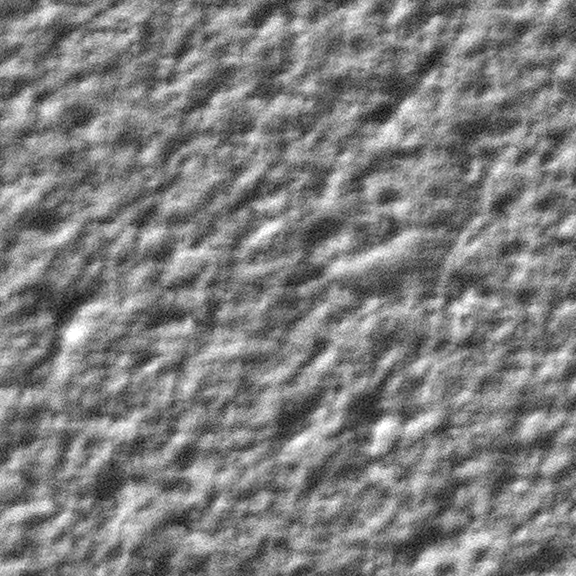
\includegraphics[width=\textwidth]{ceiling1}	
	\end{subfigure}
	~ %add desired spacing between images, e. g. ~, \quad, \qquad, \hfill etc. 
    %(or a blank line to force the subfigure onto a new line)
    \begin{subfigure}[b]{0.12\textwidth}
		\centering
		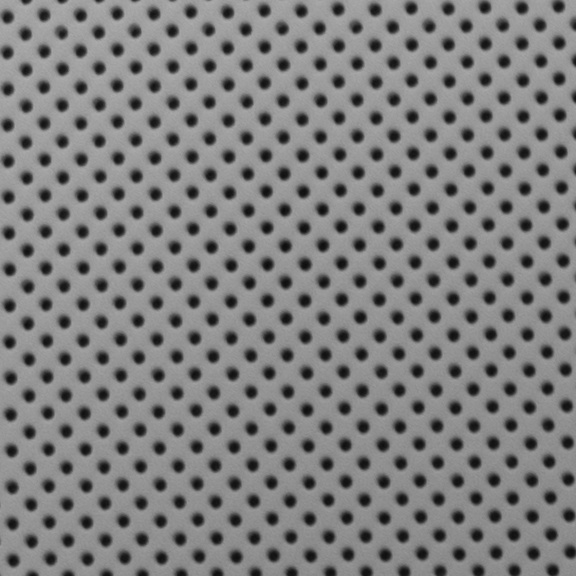
\includegraphics[width=\textwidth]{ceiling2}	
	\end{subfigure}
    ~ %add desired spacing between images, e. g. ~, \quad, \qquad, \hfill etc. 
    %(or a blank line to force the subfigure onto a new line)
    \begin{subfigure}[b]{0.12\textwidth}
		\centering
		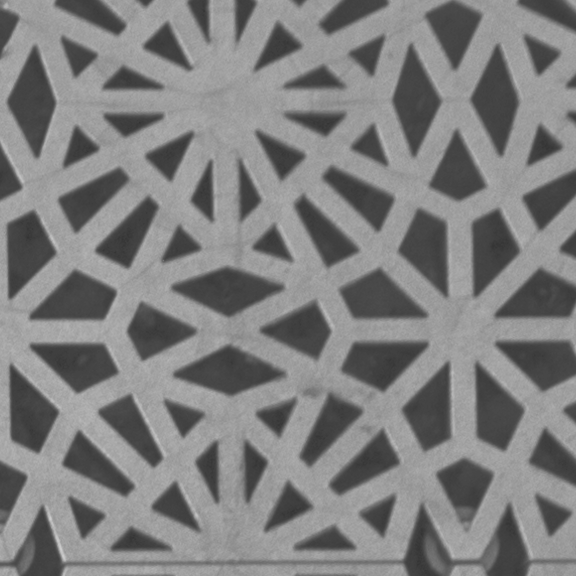
\includegraphics[width=\textwidth]{floor1}	
	\end{subfigure}
    ~ %add desired spacing between images, e. g. ~, \quad, \qquad, \hfill etc. 
    %(or a blank line to force the subfigure onto a new line)
    \begin{subfigure}[b]{0.12\textwidth}
		\centering
		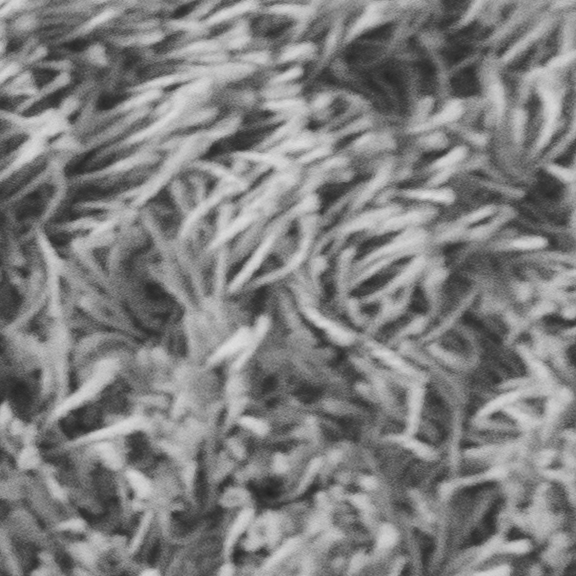
\includegraphics[width=\textwidth]{rug}	
	\end{subfigure}
    ~ %add desired spacing between images, e. g. ~, \quad, \qquad, \hfill etc. 
    %(or a blank line to force the subfigure onto a new line)
    \begin{subfigure}[b]{0.12\textwidth}
		\centering
		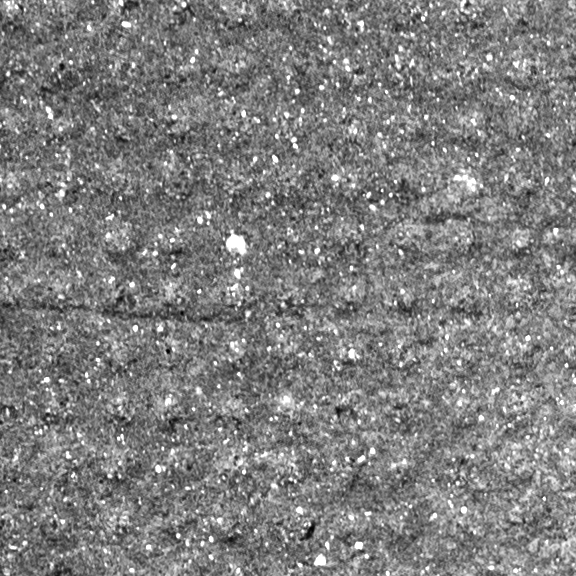
\includegraphics[width=\textwidth]{stoneslab}	
	\end{subfigure} \\[2ex]
    
        
    \begin{subfigure}[b]{0.12\textwidth}
		\centering
		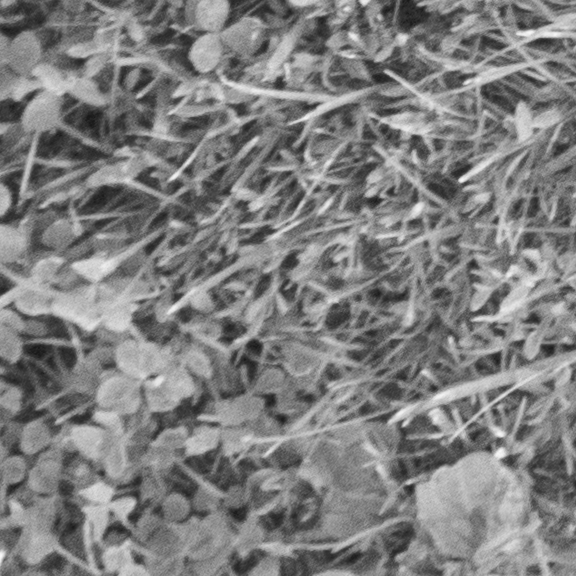
\includegraphics[width=\textwidth]{grass}	
	\end{subfigure}
	~ %add desired spacing between images, e. g. ~, \quad, \qquad, \hfill etc. 
    %(or a blank line to force the subfigure onto a new line)
    \begin{subfigure}[b]{0.12\textwidth}
		\centering
		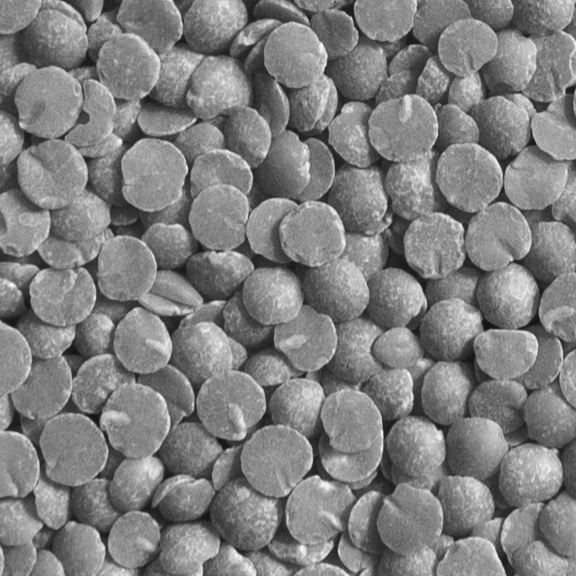
\includegraphics[width=\textwidth]{lentils}	
	\end{subfigure}
    ~ %add desired spacing between images, e. g. ~, \quad, \qquad, \hfill etc. 
    %(or a blank line to force the subfigure onto a new line)
    \begin{subfigure}[b]{0.12\textwidth}
		\centering
		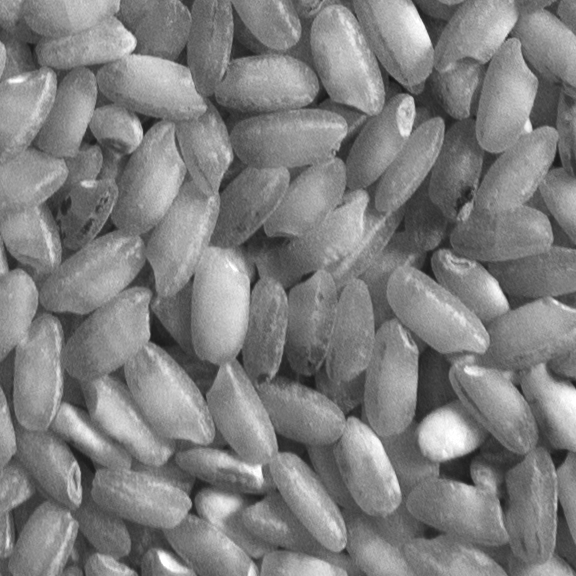
\includegraphics[width=\textwidth]{rice2}	
	\end{subfigure}
	~ %add desired spacing between images, e. g. ~, \quad, \qquad, \hfill etc. 
    %(or a blank line to force the subfigure onto a new line)
    \begin{subfigure}[b]{0.12\textwidth}
		\centering
		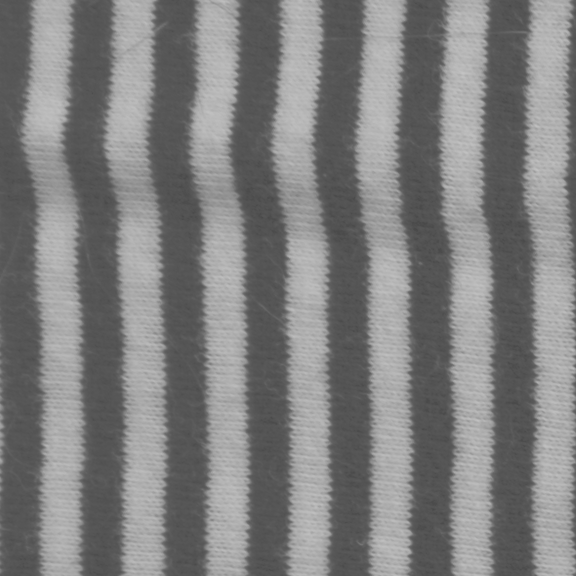
\includegraphics[width=\textwidth]{scarf2}	
	\end{subfigure}
    ~ %add desired spacing between images, e. g. ~, \quad, \qquad, \hfill etc. 
    %(or a blank line to force the subfigure onto a new line)
    \begin{subfigure}[b]{0.12\textwidth}
		\centering
		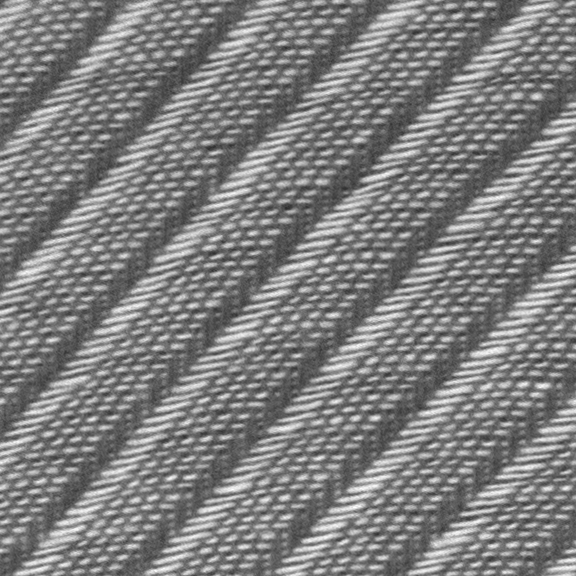
\includegraphics[width=\textwidth]{screen}	
	\end{subfigure}
    ~ %add desired spacing between images, e. g. ~, \quad, \qquad, \hfill etc. 
    %(or a blank line to force the subfigure onto a new line)
    \begin{subfigure}[b]{0.12\textwidth}
		\centering
		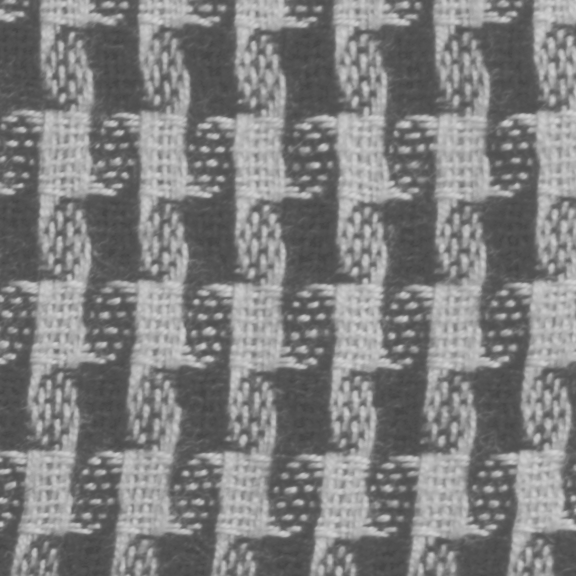
\includegraphics[width=\textwidth]{scarf1}	
	\end{subfigure}
    ~ %add desired spacing between images, e. g. ~, \quad, \qquad, \hfill etc. 
    %(or a blank line to force the subfigure onto a new line)
    \begin{subfigure}[b]{0.12\textwidth}
		\centering
		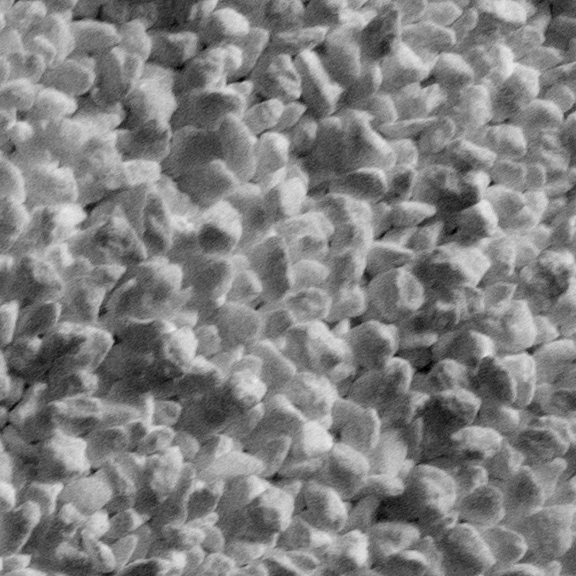
\includegraphics[width=\textwidth]{pearlsugar}	
	\end{subfigure}
		
    \caption{Some samples from the color and texture databases}
    \label{fig:databases}
\end{figure}

We compare the performance of six out of the eight measures described in section \ref{sec:measures} in the following way. First, we divide the database samples into \textit{model images} and \textit{query images}; each class only has one model and one query image. We take an image of the query set and compare its color/texture distribution (source distribution) with the color/texture distribution of all model images (target distributions). Then, we order the images from the most similar to the most dissimilar image. We repeat this process for all the images in the query set\footnote{The image classification systems (color-based and texture-based) and the datasets used for this chapter are available at \url{https://github.com/CVMethods/image_clasifier.git}}.
 
\textbf{Image color distribution.
}We use 3D histograms to represent the distribution of color pixels. Since the superhero images are very simple and do not present significant challenges, i.e., the images possess a very distinctive color palette and do not present textures or important changes in lighting, any similarity measure should be sufficient to perform the image retrieval. However, image retrieval systems are sensitive to the representation and quantification of the color image pixels. We show this effect by varying the color space and the color quantization level in the image classifier. For the color space, we represent the images in the RGB, HSL, and LAB color spaces. For the color quantization level, we represent the color space in histograms of 8, 16 and 32 bins per channel.

\textbf{Image texture distribution.} We use a family of Gabor filters as texture descriptors to obtain a distribution (2D histograms) that models the texture of the images. This type of filters models the behavior of the human visual cortex \citep{Daugman:TASSP:1988}, so they are very useful in computer vision applications to represent textures. \citep{Lee:PAMI:1996}. The family of Gabor descriptors is represented by the mother wavelet
\begin{eqnarray}
 \mathcal{G}(x,y,\omega,\theta) = \frac{\omega^2}{4\pi\kappa^2} e^{-\frac{\omega^2}{8\kappa^2}\left(4\hat{x}^2 + \hat{y}^2\right)} \cdot [e ^{i \kappa \hat{x}} -e ^ {\frac{\kappa ^ 2}{2}} ]  \label{eq:gabor_filters}
\end{eqnarray}
where $\hat{x} = x \cos \theta +  y \sin \theta$ and $\hat{y} = -x\sin \theta + y \cos \theta$ . The 2D texture histograms are a function of the energies of the Gabor responses according to the frequency $\omega$, the orientation $\theta$ and the constant $\kappa$ in the Gabor wavelet. For example, a histogram with $\kappa \approx \pi$ and 6 bins means that there are 6 different frequencies to a bandwidth of one octave and 6 different orientations. The energy of a Gabor response is given by, 
\begin{eqnarray} 
 E_{\omega,\theta} = \sum\nolimits_{x, y}|W_{x,y,\omega,\theta}|^2 \label{eq:g_energy}
\end{eqnarray}
where $W_{x,y,\omega,\theta}$ is the response of the convolution of a 2D wavelet with frequency $\omega$ and orientation $\theta$ with an image. 

\subsubsection{Image Retrieval Systems Evaluation} \label{subsubsec:evaluation}

We create a comparison benchmark for the six similarity measures. First, we normalize the distances given by the different methods between $0$ and $1$, where a value close to $0$ means the distribution the most similar to the source distribution and 1 the most dissimilar. Then we transform the normalized distances into probabilities using a softmax function $SM(\mathbf{d}) = \frac{e^{\mathbf{d}}}{\sum_{i}e^{d_i}}$. The vector $\mathbf{d}=\{d_i\}$, $\forall i=\{1, \ldots, m\}$, represents the distances between the query image to the $m$ images in the database. Considering the softmax function of the distances vector as a classification probability $SM(\mathbf{d})=\mathbf{\hat{y}}$,  we compute the cross-entropy \citep{Bishop:BOOK:2006} considering the classification ground truth $\mathbf{y}$. 
\begin{eqnarray}
H(\mathbf{y}, \mathbf{\hat{y}}) = - \sum\nolimits_{i}{y_i}\log \hat{y}_i
\label{eq:cross-entropy}
\end{eqnarray}

We can interpret the cross-entropy value as the confidence level of the image classifier for some given metric, feature space (color or texture) and histogram size. When this value is very close to zero, it indicates a perfect classification of the query image. In Fig. \ref{fig:cross_entropy}, we note the superiority of the EMD over the other measures in both color and texture-based classifiers.

\begin{figure}[ht]
    \centering
    \begin{subfigure}[b]{0.48\textwidth}
		\centering
		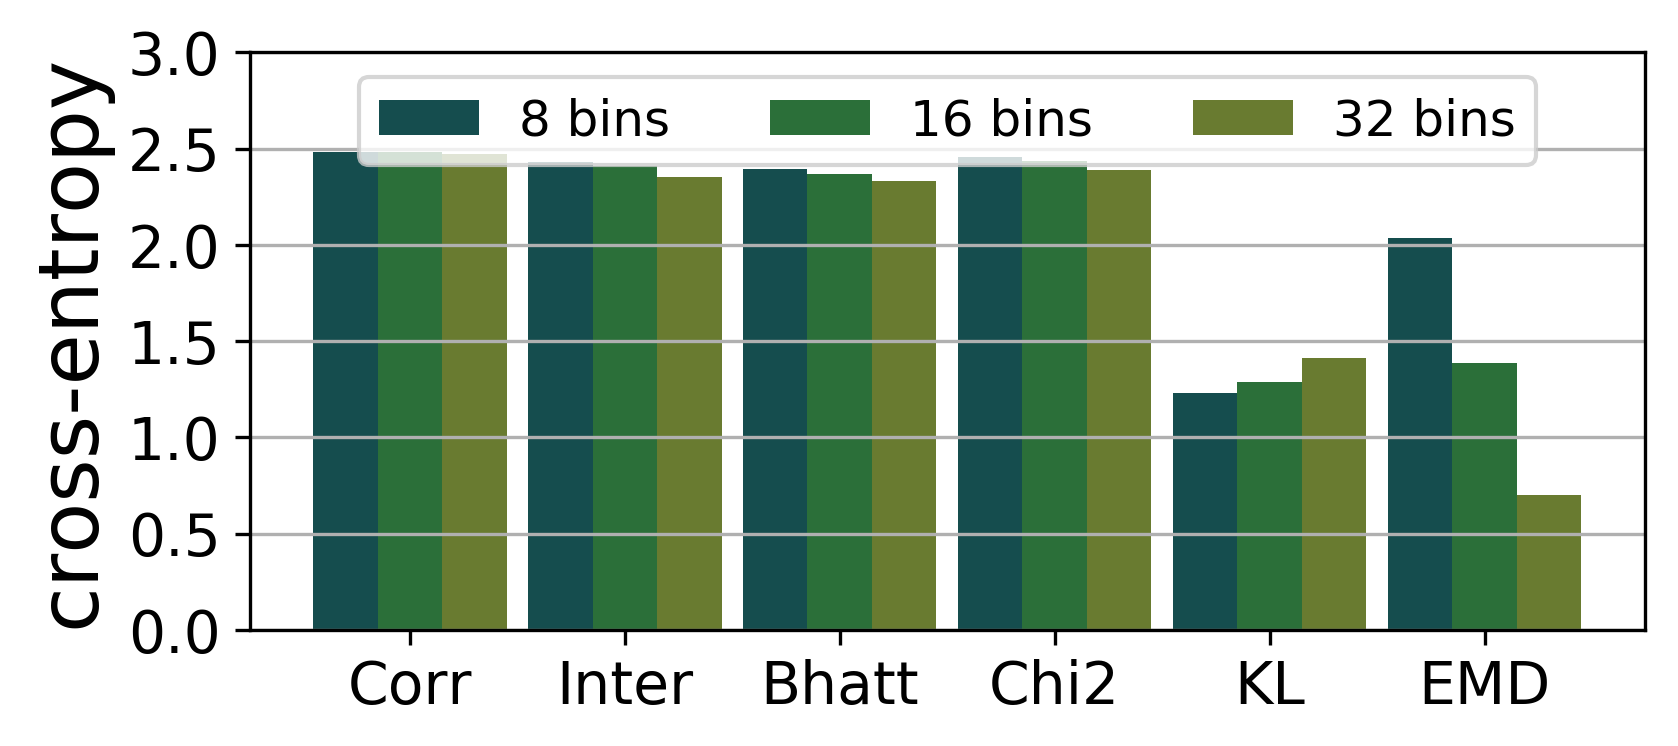
\includegraphics[width=\textwidth]{log_loss_rgb}	
		\caption{RGB color space}
	\end{subfigure}
    ~ %add desired spacing between images, e. g. ~, \quad, \qquad, \hfill etc. 
    %(or a blank line to force the subfigure onto a new line)
    \begin{subfigure}[b]{0.48\textwidth}
		\centering
		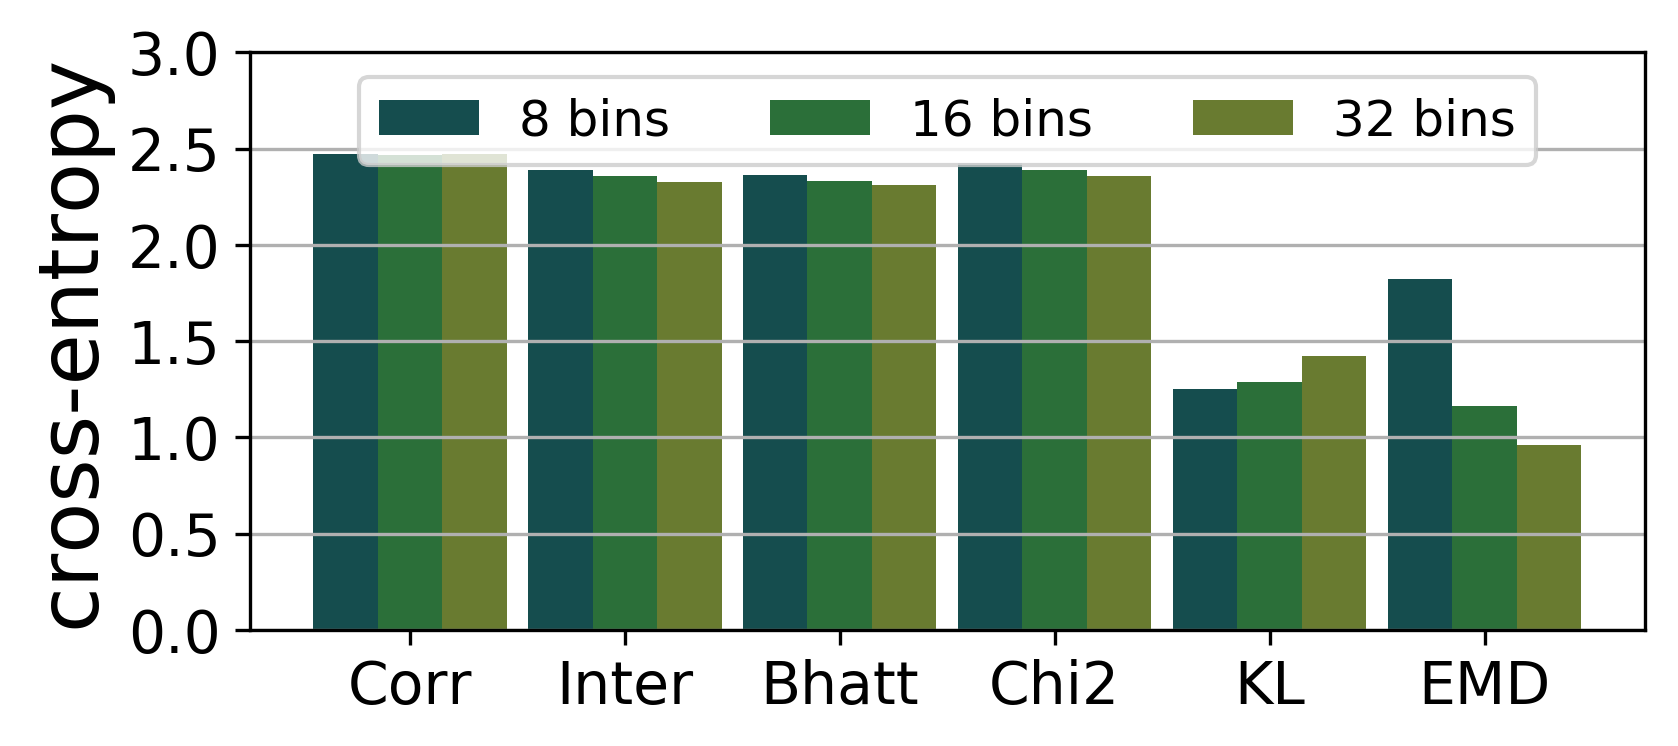
\includegraphics[width=\textwidth]{log_loss_hls}	
		\caption{HLS color space}
	\end{subfigure}\\[2ex]
	
	
    \begin{subfigure}[b]{0.48\textwidth}
		\centering
		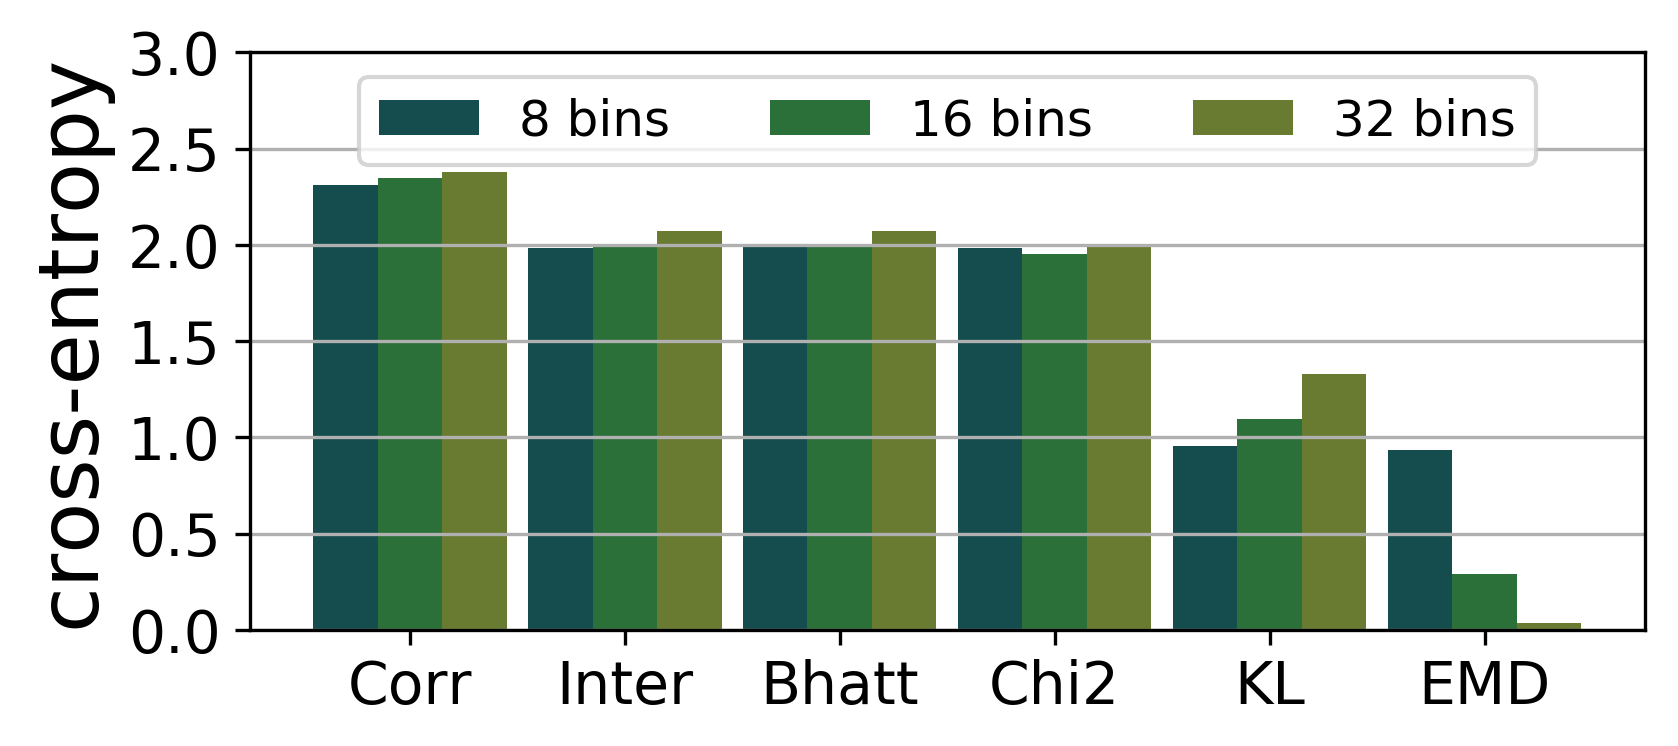
\includegraphics[width=\textwidth]{log_loss_lab}	
		\caption{LAB color space}
	\end{subfigure}   
    ~ %add desired spacing between images, e. g. ~, \quad, \qquad, \hfill etc. 
    %(or a blank line to force the subfigure onto a new line)
    \begin{subfigure}[b]{0.48\textwidth}
		\centering
		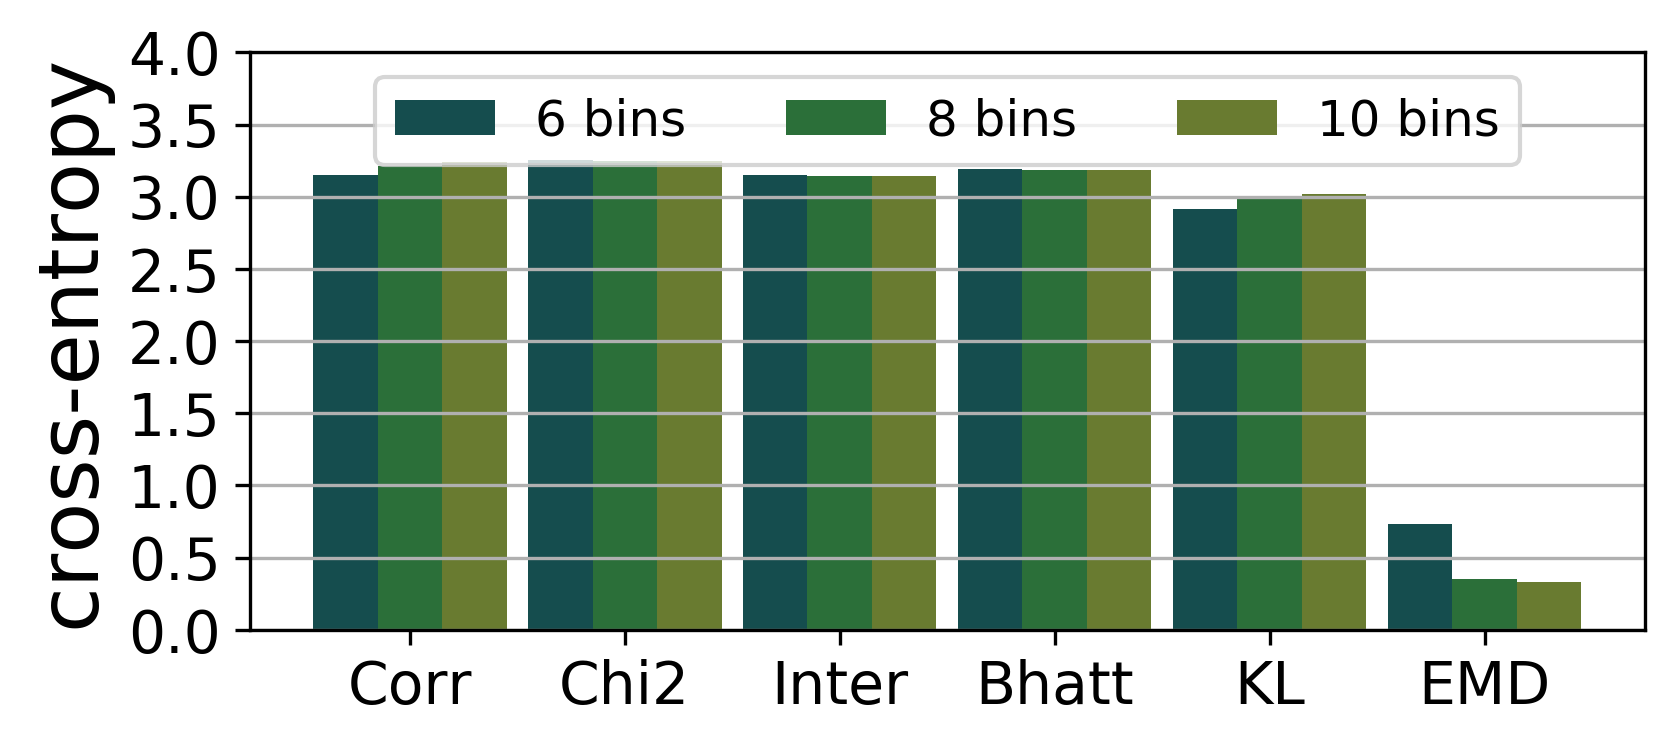
\includegraphics[width=\textwidth]{log_loss_texture}	
		\caption{Texture Gabor energy space (Eq. \ref{eq:g_energy})}
	\end{subfigure}  
		
	\caption{Cross entropy value of image retrieval systems (color and texture) using different similarity measures}
	\label{fig:cross_entropy}
\end{figure}

With the image retrieval systems, we can highlight interesting aspects of the EMD and the use of bin-to-bin measures in the comparison of distributions. First, we see the importance of the selection of the color space and the compression level of the feature space (histogram size). The effect of discretization in the bin-to-bin measures is counter-intuitive by the fact that the error increases slightly when the number of bins increases. The explanation could be a poorer intersection of mass distributions. In the case of EMD, increasing the number of bins improves the classification result. Besides, as expected, in the color-based classifier the calculation of the EMD in the LAB color space is better than in the HLS or the RGB. This effect is because the LAB color space models the color human perception in the Euclidean space, therefore, the \textit{ground distance} between two colors is easily calculated with the $L_2$ norm. On the other hand, in the texture-based classifier, we see that increase the number of bins beyond 8 bins does not improve the classification considerably. This is because the histograms with 8 frequencies and 8 orientations represent sufficiently well the image textures. 

\subsection{Texture Projection Quality Evaluation} \label{subsec:mds}

We use the multidimensional scaling (MDS) technique \citep{Kruskal:Psycho:1964} as the last evaluation test for the similarity measures on the texture dataset. The MDS allows to geometrically represent $n$ textures by a set of $n$ points $\{x_1, \ldots, x_n\}$ in a reduced Euclidean space $\mathbb{R}^{d}$, so that the distances between the points $\hat{d}_{ij} = ||x_i-x_j||_2$ correspond as much as possible to the values of dissimilarity $d_{ij}$ between the texture distributions. To evaluate the quality of the projection, we use the stress value proposed in \citep{Kruskal:Psycho:1964}.
\begin{eqnarray}
S= \sqrt{\frac{\sum_{ij}(\hat{d}_{ij}-d_{ij})^2}{\sum_{ij}\hat{d}_{ij}^2}}
\label{eq:stress}
\end{eqnarray}

The stress coeficient is a positive value that indicates how well the distances given by the measures are preserved in the new low-dimensional space, i.e. the lower the level of $S$, the better the representation of texture in a low-dimensional space (2D in our case). The figure \ref{fig:stress} shows how the lowest stress is obtained using the EMD. This is because the MDS technique interprets the distances of the entrance towards distances in a space of low dimension. Given that the EMD is the only measure that is a true metric, not only is the stress level low, but the visual projection is in accordance with the frequency $\omega$ and orientation $\theta$ used in the Gabor filters (Eq. \ref{eq:gabor_filters}) that model the distribution of the textures (see Fig. \ref{fig:MDS_EMD} in supplemental materials file).

\begin{figure}[!ht]
    \centering
    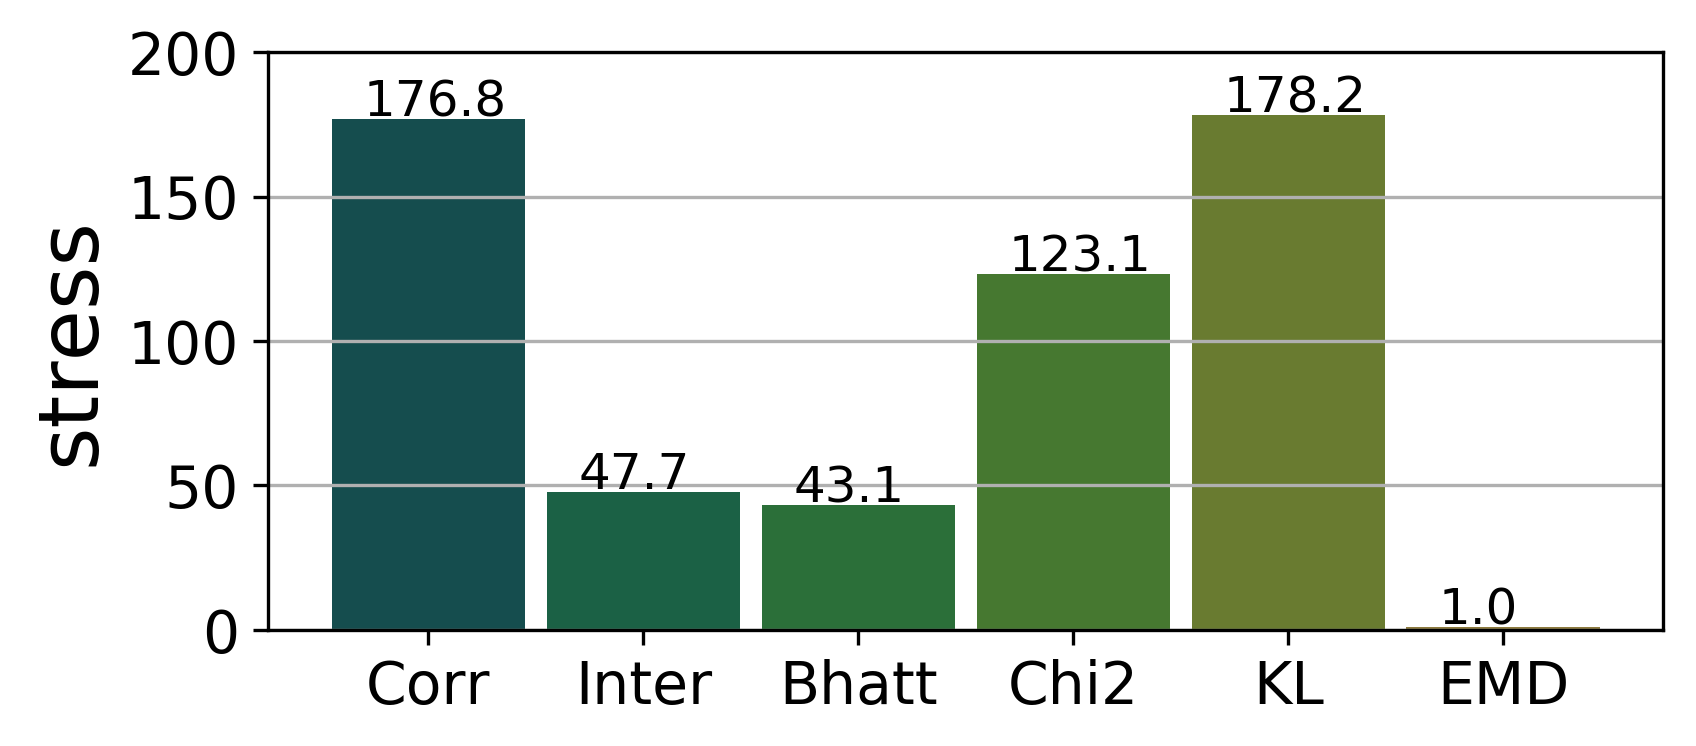
\includegraphics[width=0.45\textwidth]{stress}
 \caption{Stress value of the MDS projections using the six principal similarity measures}
 \label{fig:stress}
\end{figure}
 
\section{Conclusion}\label{sec:conclusions}

In this chapter, we compare some of the so-popular bin-to-bin similarity measures with the EMD. We measure their performance in three tests: a one-dimensional analysis with synthetic distributions, with two image classifiers (color and texture-based) and a visual projection using the MDS technique and the stress as the comparison value. The objective is to show that such measures highly used in the literature to develop complex tasks are not the best choice since they fail even in the most straightforward conditions. We illustrate that the EMD is a true metric \citep{Peyre.Cuturi:arXiv:2018} that expresses the dissimilarity between distributions naturally.

\textbf{Results.}
The experiments of the previous sections show the superiority of the EMD to represent the similarity between distributions. First, the one-dimensional case shows how the bin-to-bin measures saturate (or fall to zero) as soon as the probabilities have empty intersection (see Fig. \ref{fig:source_target_dist}). As for the image retrieval systems, we can see that by correctly choosing the feature image space and a good compression resolution of the distributions (LAB color space with 32 bins in the color-based system and the Gabor energy with 8 bins in the texture-based system), the EMD performs a perfect classification. However, this is not the case of the other measures because they are not a true distance. Representing the textures in the Euclidean space using the MDS technique, shows another advantage of the EMD. The use of the ground distance $\textbf{C}$ in the calculation of the optimal transport, making it possible to transfer 2D texture histograms to a logarithmic-polar space, making the stress value relatively low. To see some examples of the color-based image retrieval system and the 2D texture projections consult the file with supplementary material.

%\textbf{Furute Work.} Use of the metric for perceptual-based segmentation where the ground distance can be used to set specific weights for different measures like color, texture, intensity, contrast. This cannot be done without a ground distance.

\textbf{Notes about EMD computation complexity.}
We believe that EMD is a depreciated metric only because of excessive calculation time. In the examples developed before, we calculate the EMD using the iterative process of linear programming. Despite this, the calculation is fast enough to develop the image classifier. In comparison with the first EMD algorithm \citep{Rubner.Tomasi.ea:IJCV:2000}, the progress of the computer processors allows to use the same algorithm and be competitive with the bin-to-bin measures. Moreover, a solution to the excessive complexity time and memory consumption are the regularized distances, also called Sinkhorn distances \citep{Cuturi:NIPS:2013}. This entropy-based regularization accelerates the computing time giving a close approximation of the EMD. The regularization of distances allows for creating parallelizable algorithms. 